%!TEX root = ../MasterThesis.tex

\section{Analyzing \gls{E-commerce} transactions}
\label{sec:analyze_transactions}

But just sharing the fact between the relevant stakeholders if the shipping and billing address of an order is different or not is not enough. Although this information is necessary, it is not sufficient to make a decision about suspicious transactions. Other necessary information are whether the consumer has send orders to this shipping address before, and the information about the content of the current order. Nevertheless, as mentioned in Section~\ref{sec:scope_thesis} looking at the transactions of just one of the merchants is not enough either to solve the \gls{E-commerce} fraud scenario, that this thesis focuses on. \\

Therefore the idea is to combine the transaction information from various merchants, \gls{LSP}s, \gls{PSP}s and issuers into one combined and shared information space within a collaborative system to be able to analyze if there are any orders that look extraordinary, and are likely not being made by the owner of the credit card to a certain extend. This will also mean that the proposed solution will use statistical evaluations and probabilities to find and rate suspicious activities. Starting with the credit card in question an issuer can query for the order details of all the transactions, that have been done with the credit card online recently. For that they will likely have to query the \gls{PSP}s for the payment tokens first, before asking the affected merchant for order details to any of those payment tokens. At the end each online transaction can be mapped into a schema like the one shown in Figure~\ref{fig:images_data_model}, building up a large graph of entities and  the relationships between them, and with the specific credit card in the center of it. An abbreviated sample graph of this procedure can be seen in Figure~\ref{fig:images_credit_card_graph}. \\

As shown in this figure the transactions will be clustered by merchants first. Still collecting the various order information into one combined data set is just the beginning of the \gls{E-commerce} fraud incident analysis. Based on the information received an issuer can already filter out transactions, that have been shipped to different addresses than the one the credit card owner is registered for. Especially for those edge cases it might be worth to ask for additional information from the affected merchants to figure out if that consumer has used one of these shipping addresses before. As a result the existing data set can be further enriched with supplementary transactional information from merchants at any time if needed. In addition to the address information an issuer can also analyze the item information (incl.\ category, brand and model) of each order. \\

\begin{figure}[!ht]
  \centering
  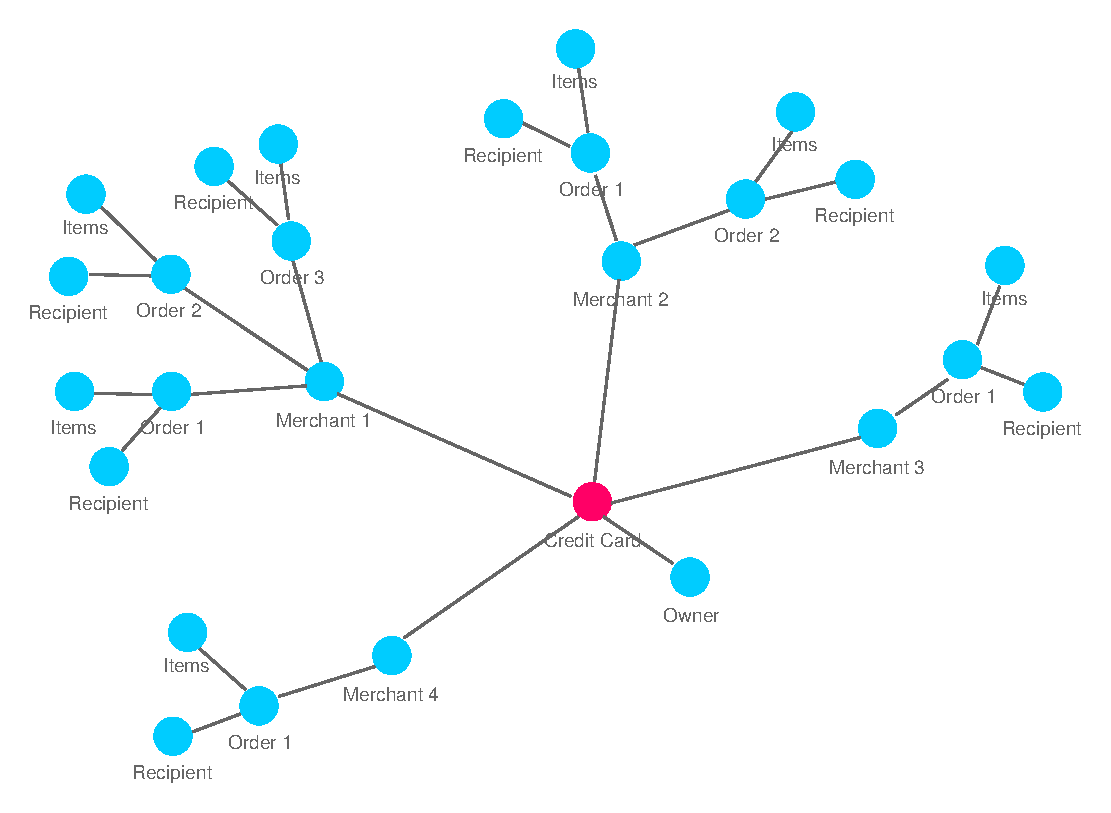
\includegraphics[width=0.9\columnwidth]{images/ontology_scenario_2.pdf}
  \caption{Building clusters of E-commerce transactions by merchant}
\label{fig:images_credit_card_graph}
\end{figure}

But as already stated, analyzing the cluster of transactions merchant by merchant will not be sufficient to come up with a solid decision about a suspicious transaction. This is mostly due to the usage pattern of the fraudsters, that have been described in the scenario selected for this Master thesis in Section~\ref{sec:scope_thesis}. Due to this scenario the various order details from the merchants have to be mapped against each other, so that the initial graph of transactions clustered by merchant can be easily transformed into complementary representations, whose use different criteria to cluster the transactions --- such as recipient addresses, branches of merchants, or product-related information. This reshaping of the graph can lead to new insights about the ``normal'' shopping behavior of a credit card owner, and can make deviations from this behavior visible. Visualizing the combined data set as a clustered graph on screen supports the exploratory nature of knowledge generation and perception, and can therefore help speed up the investigation of  \gls{E-commerce} fraud incidents. An example visualization of a clustered graph, that groups information together based on a criteria, is shown in Figure~\ref{fig:images_graph_viz}. The different colors in this figure can represent different sources of information (e.g.\ \gls{E-commerce} transactions from various merchants). In this example information that stands out from the ``normal behavior'' can be found in the lower right section of the figure. \\

\begin{figure}[!ht]
  \centering
  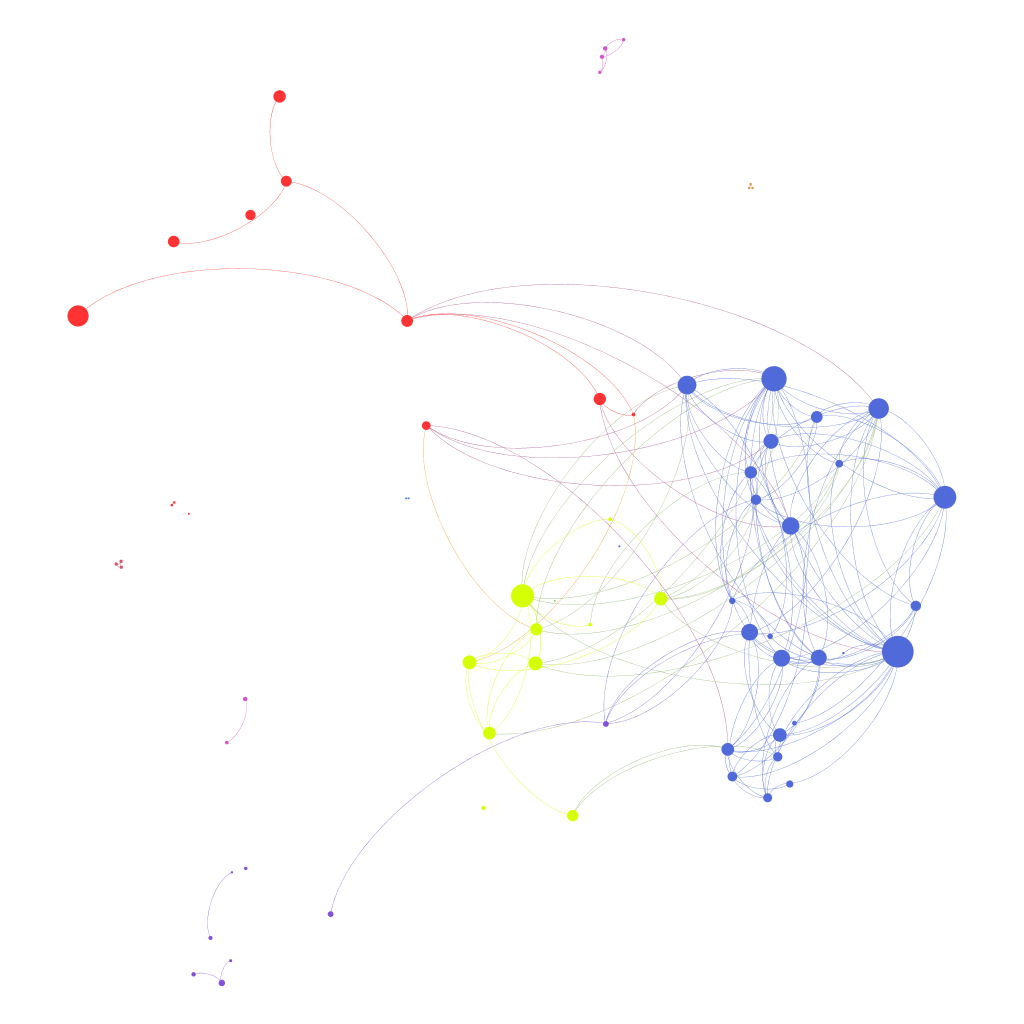
\includegraphics[width=0.9\columnwidth]{images/GraphViz.png}
  \caption[An example visualization of a clustered graph]{An example visualization of a clustered graph \citep{visjsshowcase}}
\label{fig:images_graph_viz}
\end{figure}

 In addition to these clustered graphs the collaborative system can also support the \gls{E-commerce} fraud investigation by switching the type of visualization  based on the criteria chosen for the clustering of the transactions; e.g.\ when clustering them based on location information such as shipping addresses the system can present the information as a heat map on a chart as is displayed in Figure~\ref{fig:images_map_heatmap}. \\

\begin{figure}[!ht]
  \centering
  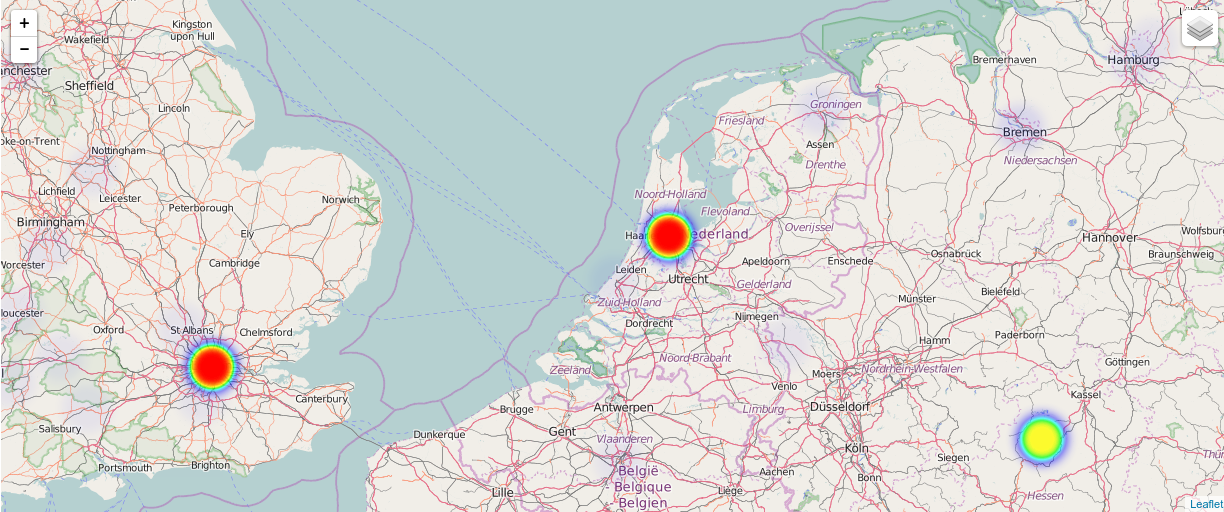
\includegraphics[width=0.9\columnwidth]{images/Heatmap.png}
  \caption{Heatmap displaying clusters of location-based information}
\label{fig:images_map_heatmap}
\end{figure}

To conclude the system have to support the collection and combination of \gls{E-commerce} transaction information from various sources into a large clustered graph, that can be analyzed from multiple view points to validate, if there are any transactions that stand out from the ``normal'' shopping behavior of the credit card owner. The starting point for the investigation is a sequence of recent credit card activities, that an issuer can provide to the other participants. The graph will initially collect and cluster the information from each merchant based on this list. In case there are suspicious information in one of the transaction clusters of each merchant, an issuer can ask for further details and enrich that specific cluster with additional order information for this consumer and that merchant. In the final step the system has to do the mapping of the order detail information between each merchant to allow subsequent analyzing and clustering of the transactions with different criteria.

% section system_overview (end)
